\chapter{Conducted Experiments}\label{chap:exp}

In this chapter, we outline all experiments and discuss the results.
We end up with two best performing models --- Na\"{\i}ve Bayes and decision tree.
Maybe somewhat surprisingly, those models do not make use of any word features,
but exploit only high-level features.

Our original intention was to try all combinations of features, feature selection and classifiers.
However, this turned out to be computationally infeasible.
Instead, we tried promising subsets by choosing the best variant out of each round.

The final dataset used for experiments contains  64,550 instances.
We used 10-fold crossvalidation --- each split had
58,095 training and 6,455 testing instances.
The exact format of the dataset can be found in \Cref{app:dataset}.

We report accuracy and f-measure.
Because every classifier was trained and tested 10 times,
we report the arithmetic mean as the representative value of the classifier
together with minimum, maximum and standard deviation.
As it can be seen from the tables bellow, 
the values were fairly stable with low standard deviation and
as such should be reasonably reliable.

We performed the analysis in five rounds.
We report f-measure and accuracy of all models to retain comparability even throughout rounds.
Each round focuses on a different variable as listed bellow:

\begin{enumerate}
	\item baseline
	\item feature sets with Na\"{\i}ve Bayes
	\item feature selection algorithms
	\item classifiers
	\item size of training data
\end{enumerate}


\section{1st round --- Baseline}

In this round, we ran zero-R and one-R to get an idea about the problem.

Zero-R achieves accuracy of 70\% as reported in \Cref{tab:base_perf}.
This is in compliance with the label distribution,
because the dataset contains approximately the same proportion of not-useful instances.
One-R raises this performance a bit to 73\%.

Because zero-R assigns all instances label \textit{not-useful},
there are no true positive instances.
Hence precision and recall are zero.
For this reason, f-measure is undefined for zero-R.
We can take one-R for f-measure baseline (56\%).

\begin{table}[h!]

\centering
\begin{tabular}{lr@{~}r@{~}rr@{~}r@{~}r}
\toprule
\textbf{name}	& \multicolumn{3}{c}{\textbf{f-measure}} & \multicolumn{3}{c}{\textbf{accuracy}} \\
\midrule
zero-R & \multicolumn{3}{c}{N/A} & 0.70 & (0.69, 0.70) & $\pm$ 0.004 \\
one-R & 0.56 & (0.54, 0.58) & $\pm$ 0.012 & 0.73 & (0.72, 0.74) & $\pm$ 0.005 \\

\bottomrule
\end{tabular}

\caption{Performance of Feature Selections}\label{tab:base_perf}
All reported values are in the format `arithmetic mean (min, max) $\pm$ standard deviation'.
\end{table}

\section{2nd round --- Features}

In this round, we run Na\"{\i}ve Bayes with different sets of features.
Configurations with results are shown in \Cref{tab:feat_perf}.
Names refer to feature sets.
\textbf{\{uni,bi\}grams} and \textbf{\{uni,bi,tri\}grams} are listed n-grams together.
\textbf{basic} is STARS, REVIEWLEN, SPELLCHECK and COSINESIM.

We can clearly see that none of the feature set brought desired improvement.
Only feature set \textbf{basic} brought a 3 percent improvement in f-measure.
Other sets brought immense deterioration.
Any combination of \textbf{Bigrams} or \textbf{TF-IDF} decreased the accuracy by at least 30\%.
This is probably due to overfitting.
The feature sets contains so many features, that our model learnt to recognise
irregularities in the data.
This claim supports a brief analysis of the features showing that
even words like `in', `to' or `that,' which clearly carry no information about usefulness.
It is interesting to note that f-measure did not suffer from such a big decrease.



\begin{table}[h!]

\centering
\begin{tabular}{lr@{~}r@{~}rr@{~}r@{~}r}
\toprule
\textbf{name}	& \multicolumn{3}{c}{\textbf{f-measure}} & \multicolumn{3}{c}{\textbf{accuracy}} \\
\midrule
unigrams& 0.47 & (0.46, 0.48) & $\pm$ 0.007 & 0.30 & (0.29, 0.32) & $\pm$ 0.006 \\
tfidf& 0.47 & (0.46, 0.48) & $\pm$ 0.007 & 0.30 & (0.29, 0.32) & $\pm$ 0.006 \\
\{uni,bi\}grams	& 0.47 & (0.46, 0.47) & $\pm$ 0.005 & 0.30 & (0.30, 0.31) & $\pm$ 0.004\\
bigrams & 0.47 & (0.46, 0.47) & $\pm$ 0.005 & 0.31 & (0.30, 0.31) & $\pm$ 0.005			\\
entities & 0.48 & (0.47, 0.49) & $\pm$ 0.005 & 0.35 & (0.34, 0.36) & $\pm$ 0.005		\\
\{uni,bi,tri\}grams & 0.47 & (0.46, 0.48) & $\pm$ 0.008 & 0.30 & (0.29, 0.32) & $\pm$ 0.007	\\
trigrams & 0.47 & (0.46, 0.49) & $\pm$ 0.008 & 0.32 & (0.31, 0.33) & $\pm$ 0.006		\\
cosine\_sim & \multicolumn{3}{c}{N/A} & 0.70 & (0.69, 0.70) & $\pm$ 0.006		\\
\textbf{basic} & 0.59 & (0.58, 0.60) & $\pm$ 0.005 & 0.71 & (0.71, 0.72) & $\pm$ 0.004		\\
basic+bigrams & 0.48 & (0.47, 0.49) & $\pm$ 0.007 & 0.35 & (0.34, 0.36) & $\pm$ 0.006		\\
basic+tfidf & 0.48 & (0.47, 0.50) & $\pm$ 0.007 & 0.36 & (0.35, 0.37) & $\pm$ 0.006			\\
\textbf{basic+entities} & 0.55 & (0.54, 0.56) & $\pm$ 0.008 & 0.54 & (0.53, 0.55) & $\pm$ 0.006		\\
\bottomrule
\end{tabular}


\caption{Performance of Feature Configurations}\label{tab:feat_perf}
All reported values are in the format `arithmetic mean (min, max) $\pm$ standard deviation'.
\end{table}


\section{3rd round --- Feature Selection}

In this round, we compare three different methods of feature selection.
The attempt is to avoid the overfitting described in the previous section.
We use features \textbf{basic+entities} and Na\"{i}ve Bayes.
We run PCA with 100 dimensions as recommended by scipy documentation.
For mutual information and chi square, we choose top 1000 features.

From \Cref{tab:sel_perf}, we can see that both mutual information
and chi-square improved the accuracy to 58\% and f-measure even to the original
0.56 from the baseline.
Choosing the threshold for the number of features more carefully could improve the results even further, possible above the performance of the baseline.
We have not analyzed this due the lack of time.

PCA decreased the performance by a significant margin.
This could be due to non-optimal parameters, which
again could be improved by more careful analysis.

\begin{table}[h!]

\centering
\begin{tabular}{lr@{~}r@{~}rr@{~}r@{~}r}
\toprule
\textbf{name}	& \multicolumn{3}{c}{\textbf{f-measure}} & \multicolumn{3}{c}{\textbf{accuracy}} \\

\midrule
basic+entities & 0.55 & (0.54, 0.56) & $\pm$ 0.008 & 0.54 & (0.53, 0.55) & $\pm$ 0.006		\\
\textbf{basic+entities[MI]} & 0.56 & (0.55, 0.57) & $\pm$ 0.007 & 0.58 & (0.57, 0.60) & $\pm$ 0.008 \\
\textbf{basic+entities[CHI]} & 0.56 & (0.55, 0.57) & $\pm$ 0.007 & 0.58 & (0.57, 0.59) & $\pm$ 0.007 \\
basic+entities[PCA] & 0.47 & (0.46, 0.48) & $\pm$ 0.007 & 0.30 & (0.3, 0.31) & $\pm$ 0.006 \\


\bottomrule
\end{tabular}

\caption{Performance of Feature Selections}\label{tab:sel_perf}
All reported values are in the format `arithmetic mean (min, max) $\pm$ standard deviation'.
\end{table}

\section{4th round --- Classifiers}

In the fourth round, we decided to try different classifiers as opposed to the previously used Na\"{\i}ve Bayes.
We used the following classifiers and features:

\begin{itemize}
\item Na\"{\i}ve Bayes; \textbf{basic}
\item FastText; raw text
\item decision tree; \textbf{basic}
\end{itemize}

Na\"{\i}ve Bayes was chosen the best performing data set.
Fast Text is designed for working with raw text.
Decision tree tends to suffer from overfitting when too many features are used.
Also, the training time increases significantly with the number of features,
because mutual information needs to be computed for all features in all nodes.
Therefore, we used only feature set \textbf{basic}.

The results can be seen in \Cref{tab:clsf_perf}.
The performance of FastText was comparable to Na\"{\i}ve Bayes on \textbf{basic+entities}.


The best performance in accuracy was achieved by decision tree.
It improves the previous top performing one-R by 3\%, but decreasing the f-measure.
This is a reasonable result, since one-R is a special simpler case of decision tree.
The best performing model in terms of f-measure is Na\"{\i}ve Bayes.


\begin{table}[h!]

\centering
\begin{tabular}{lr@{~}r@{~}rr@{~}r@{~}r}
\toprule
\textbf{name}	& \multicolumn{3}{c}{\textbf{f-measure}} & \multicolumn{3}{c}{\textbf{accuracy}} \\
\midrule

Na\"{\i}ve Bayes & 0.59 & (0.58, 0.60) & $\pm$ 0.005 & 0.71 & (0.71, 0.72) & $\pm$ 0.004		\\

FastText & 0.53 & (0.52, 0.54) & $\pm$ 0.009 & 0.55 & (0.54, 0.57) & $\pm$ 0.008 \\
\textbf{Decision tree} & 0.52 & (0.49, 0.54) & $\pm$ 0.012 & 0.74 & (0.73, 0.74) & $\pm$ 0.004 \\

\bottomrule
\end{tabular}

\caption{Performance of Different Classifiers}\label{tab:clsf_perf}
All reported values are in the format `arithmetic mean (min, max) $\pm$ standard deviation'.
\end{table}


\section{5th round --- Training Size}

Lastly, we perform learning curves analysis as described in \Cref{sec:lcurves}.
Each phase of 10-fold crossvalidation produces training and testing set.
The testing set is the same for all sizes of the training set.
For the training set, subsets of the original are used in such a way that 
all smaller sets are proper subsets of any bigger.

The graphs bellow show both performance of the subset of the training set and of the full testing set.
The x axis is log scaled.
Some values of f-measure for very small sets were ignored for the same reason as with zero-R.
It is undefined as there are no true positives.

We report the two best performing models from the previous round -- Na\"{\i}ve Bayes and decision tree
with feature set \textbf{basic}.

As we can see in \Cref{fig:l_curves2_accuracy} and \Cref{fig:l_curves2_f_measure}, Na\"{\i}ve Bayes performs comparably the same on both the training and testing sets when trained
on already only as many as 100 instances.
It is very likely to generalise well as the performance is virtually identical.
Also, the performance stabilizes well as the minimal and maximal values are very close to the mean.

It is worth noting that decision tree achieves comparable performance as can be seen in
\Cref{fig:l_curves3_accuracy} and \Cref{fig:l_curves3_f_measure}.
However, it needs at least 10 000 instances to achieve so.
Na\"{\i}ve Bayes is a clear winner here as it needs a lot less instances.
It would be beneficial to plot learning curves for other models,
because it could show the reasons why our more sophisticated models with
more features performed significantly worse.
However, due to the computing complexity, we did not analyse it.
It can be the subject of further research.

From the numbers, it is clear that our models did not perform significantly better than the baseline model.
Even our best performing models achieved accuracy of only approximately 70\% which can be accomplished by labelling all instances as not-useful.
The reason could be there is not enough information in the reviews to predict
 usefulness, the inner dependency is much more complicated than what can be conveyed by our simple models or the number of useful likes is not a representative metrics.



\begin{figure}[h]\centering
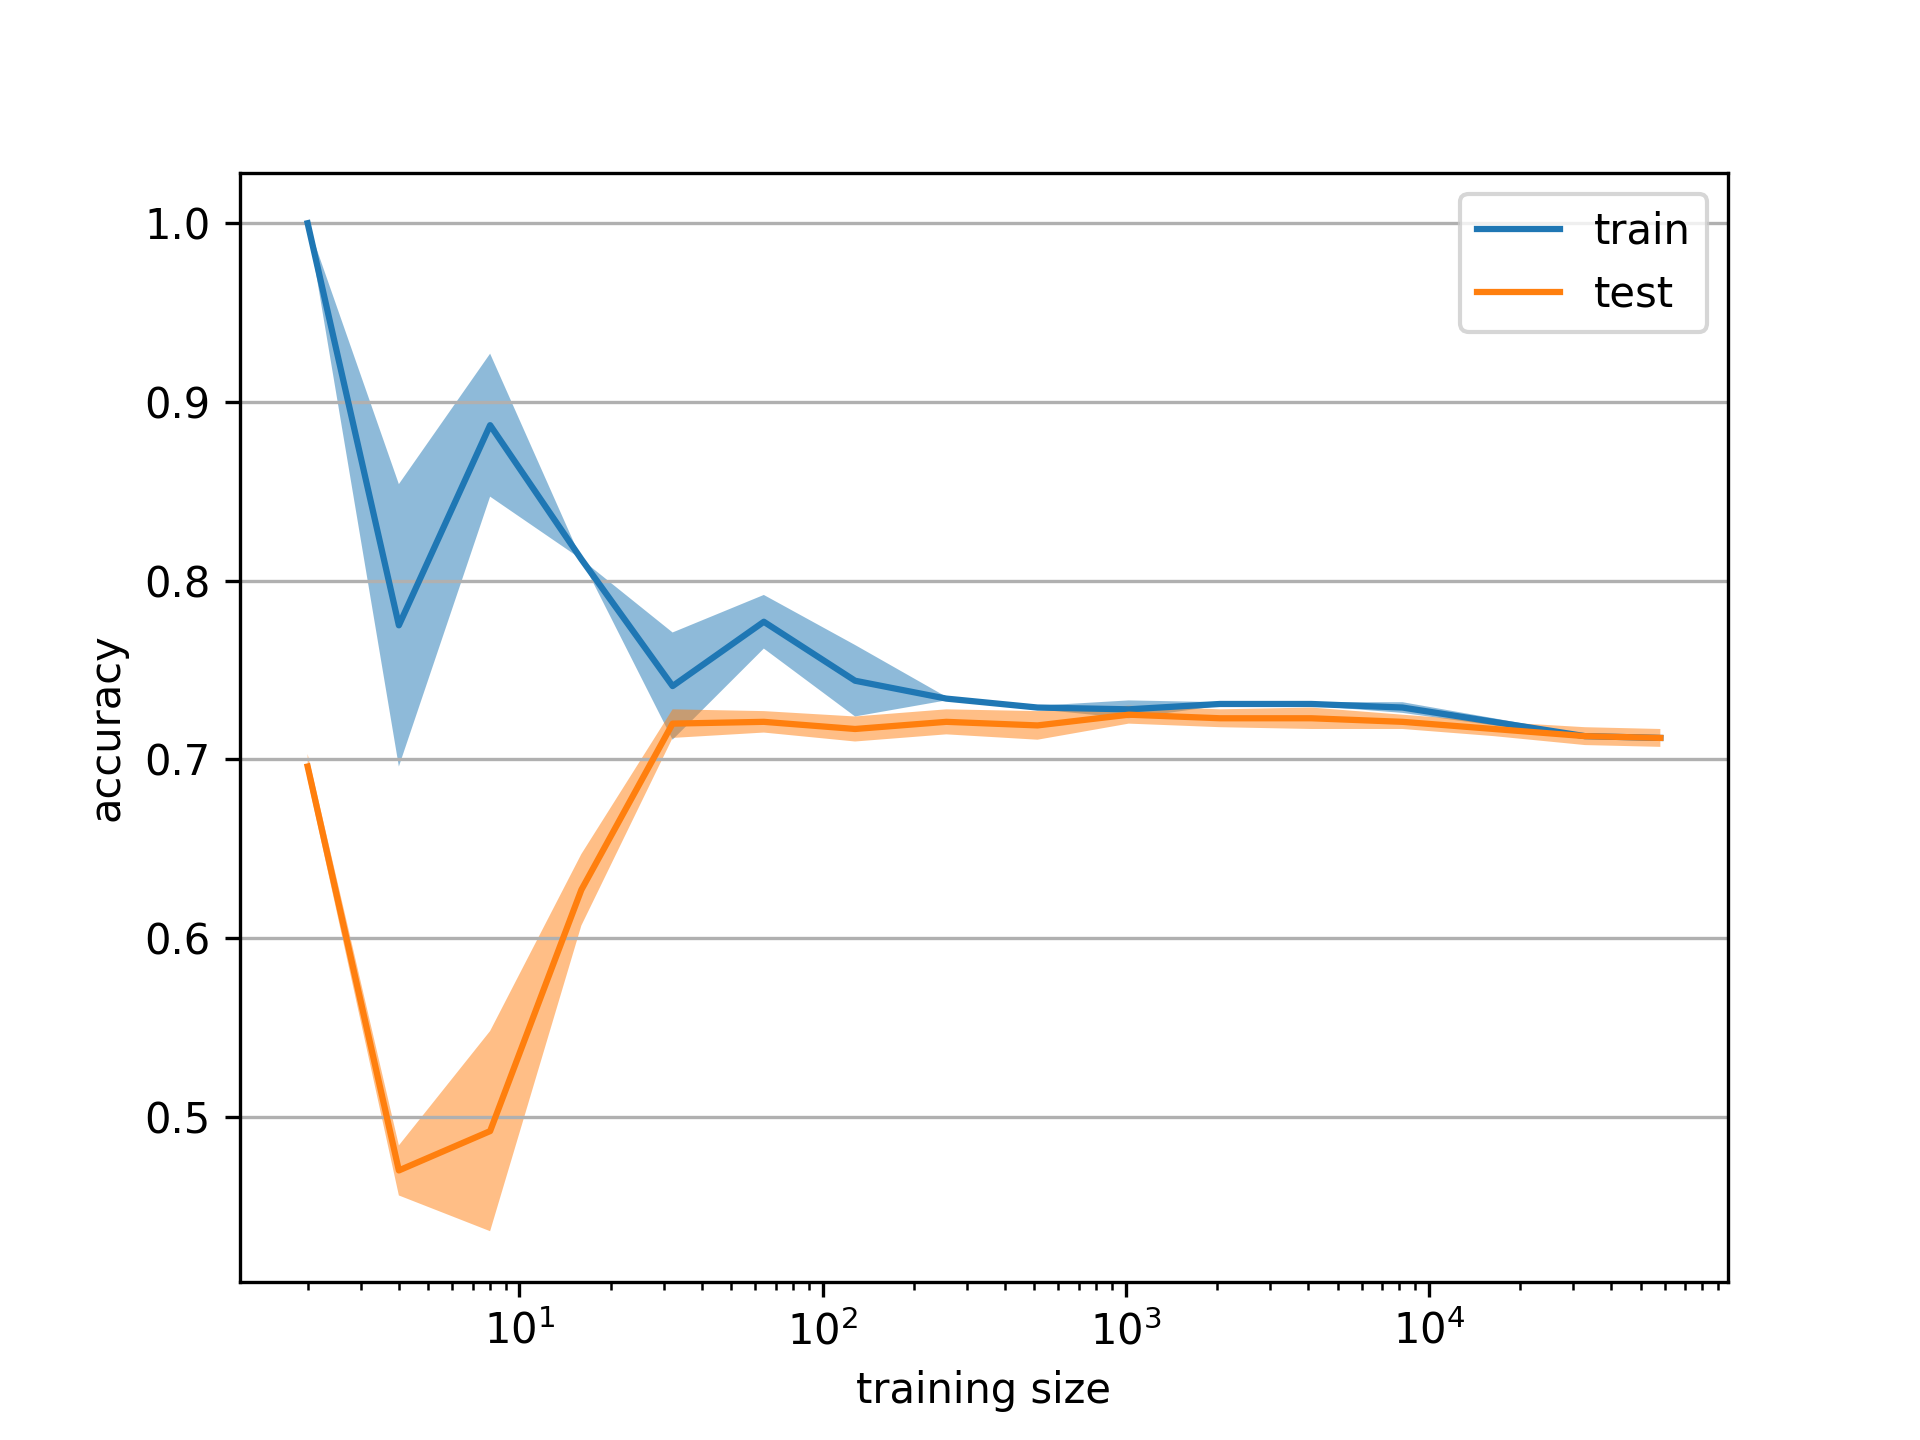
\includegraphics[width=130mm]{figures/lc2_acc.png}
\caption{Learning curves with standard deviation for Na\"{\i}ve Bayes --- accuracy}\label{fig:l_curves2_accuracy}
The x axis is log scaled.
\end{figure}

\begin{figure}[h]\centering
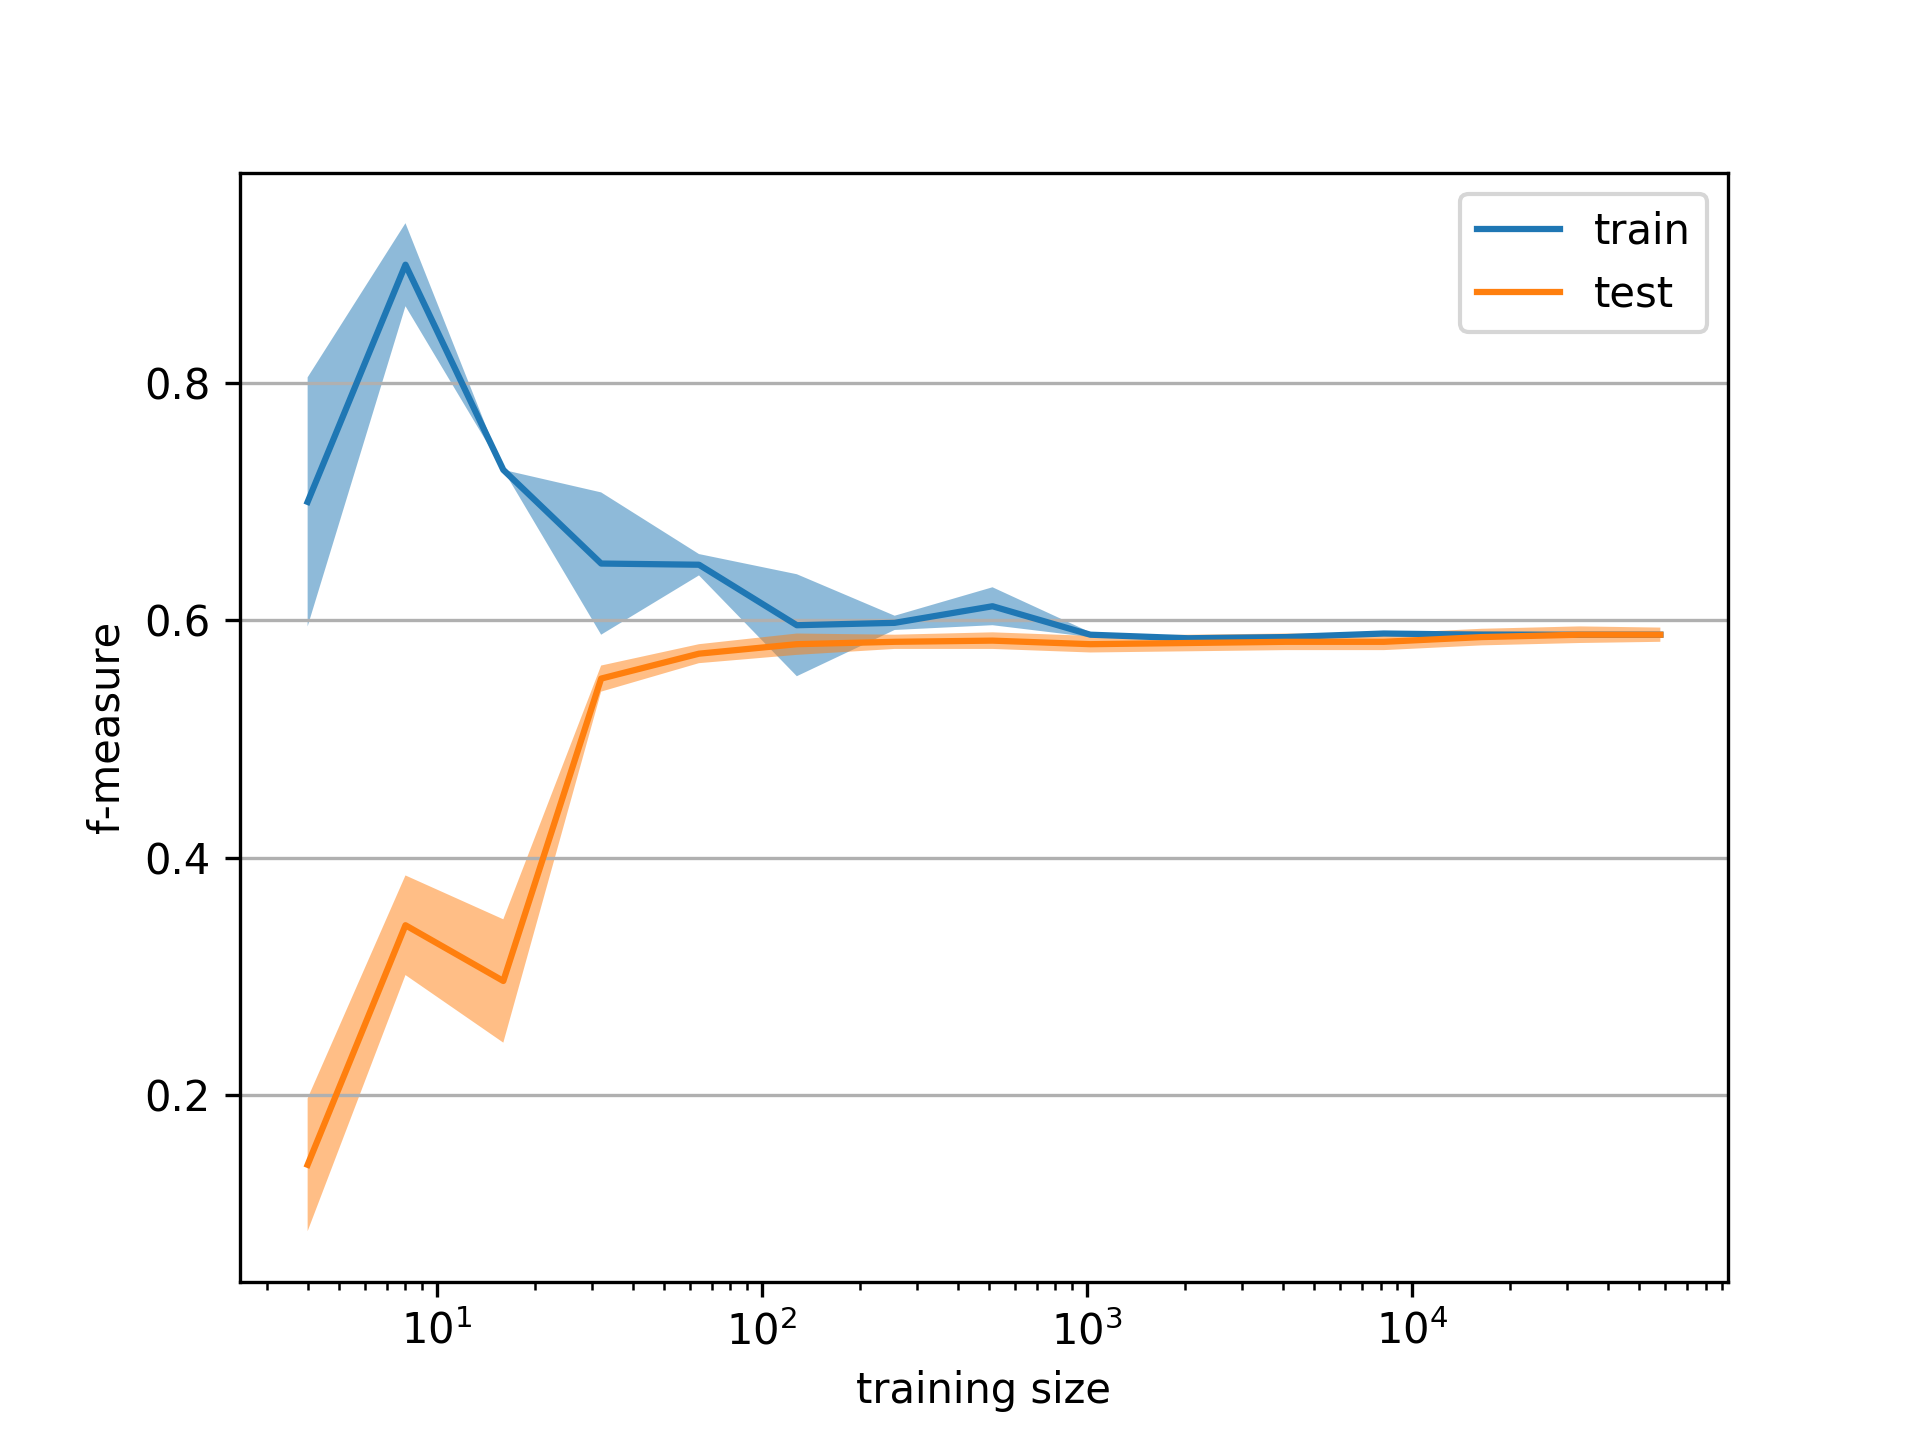
\includegraphics[width=130mm]{figures/lc2_fm.png}
\caption{Learning curves with standard deviation for Na\"{\i}ve Bayes --- f-measure}\label{fig:l_curves2_f_measure}
The x axis is log scaled.
\end{figure}


\begin{figure}[h]\centering
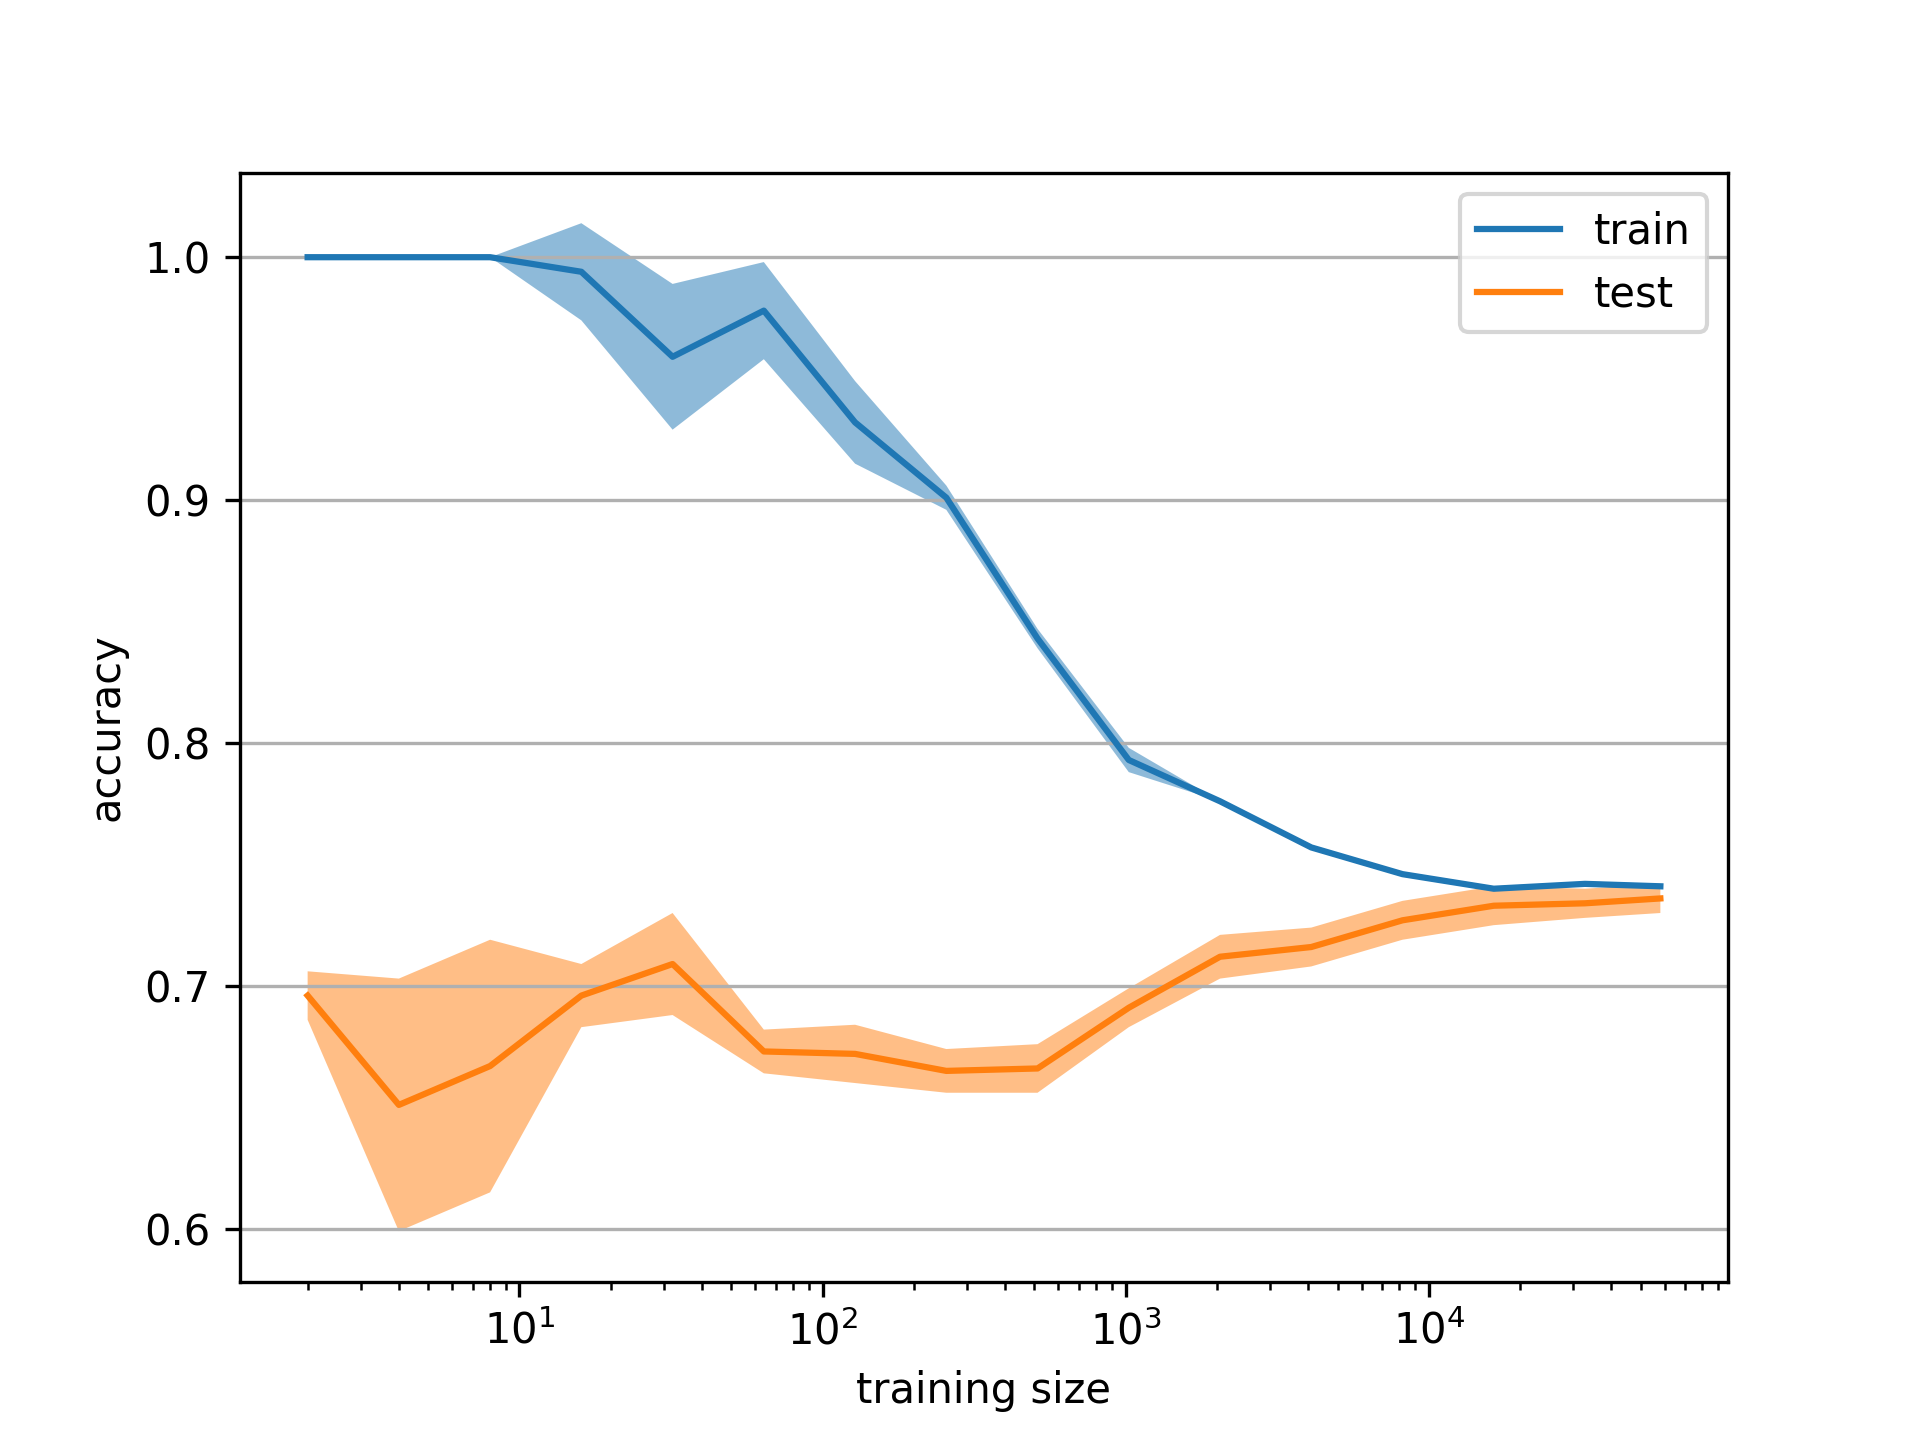
\includegraphics[width=130mm]{figures/lc3_acc.png}
\caption{Learning curves with standard deviation for decision tree --- accuracy}\label{fig:l_curves3_accuracy}
The x axis is log scaled.
\end{figure}

\begin{figure}[h]\centering
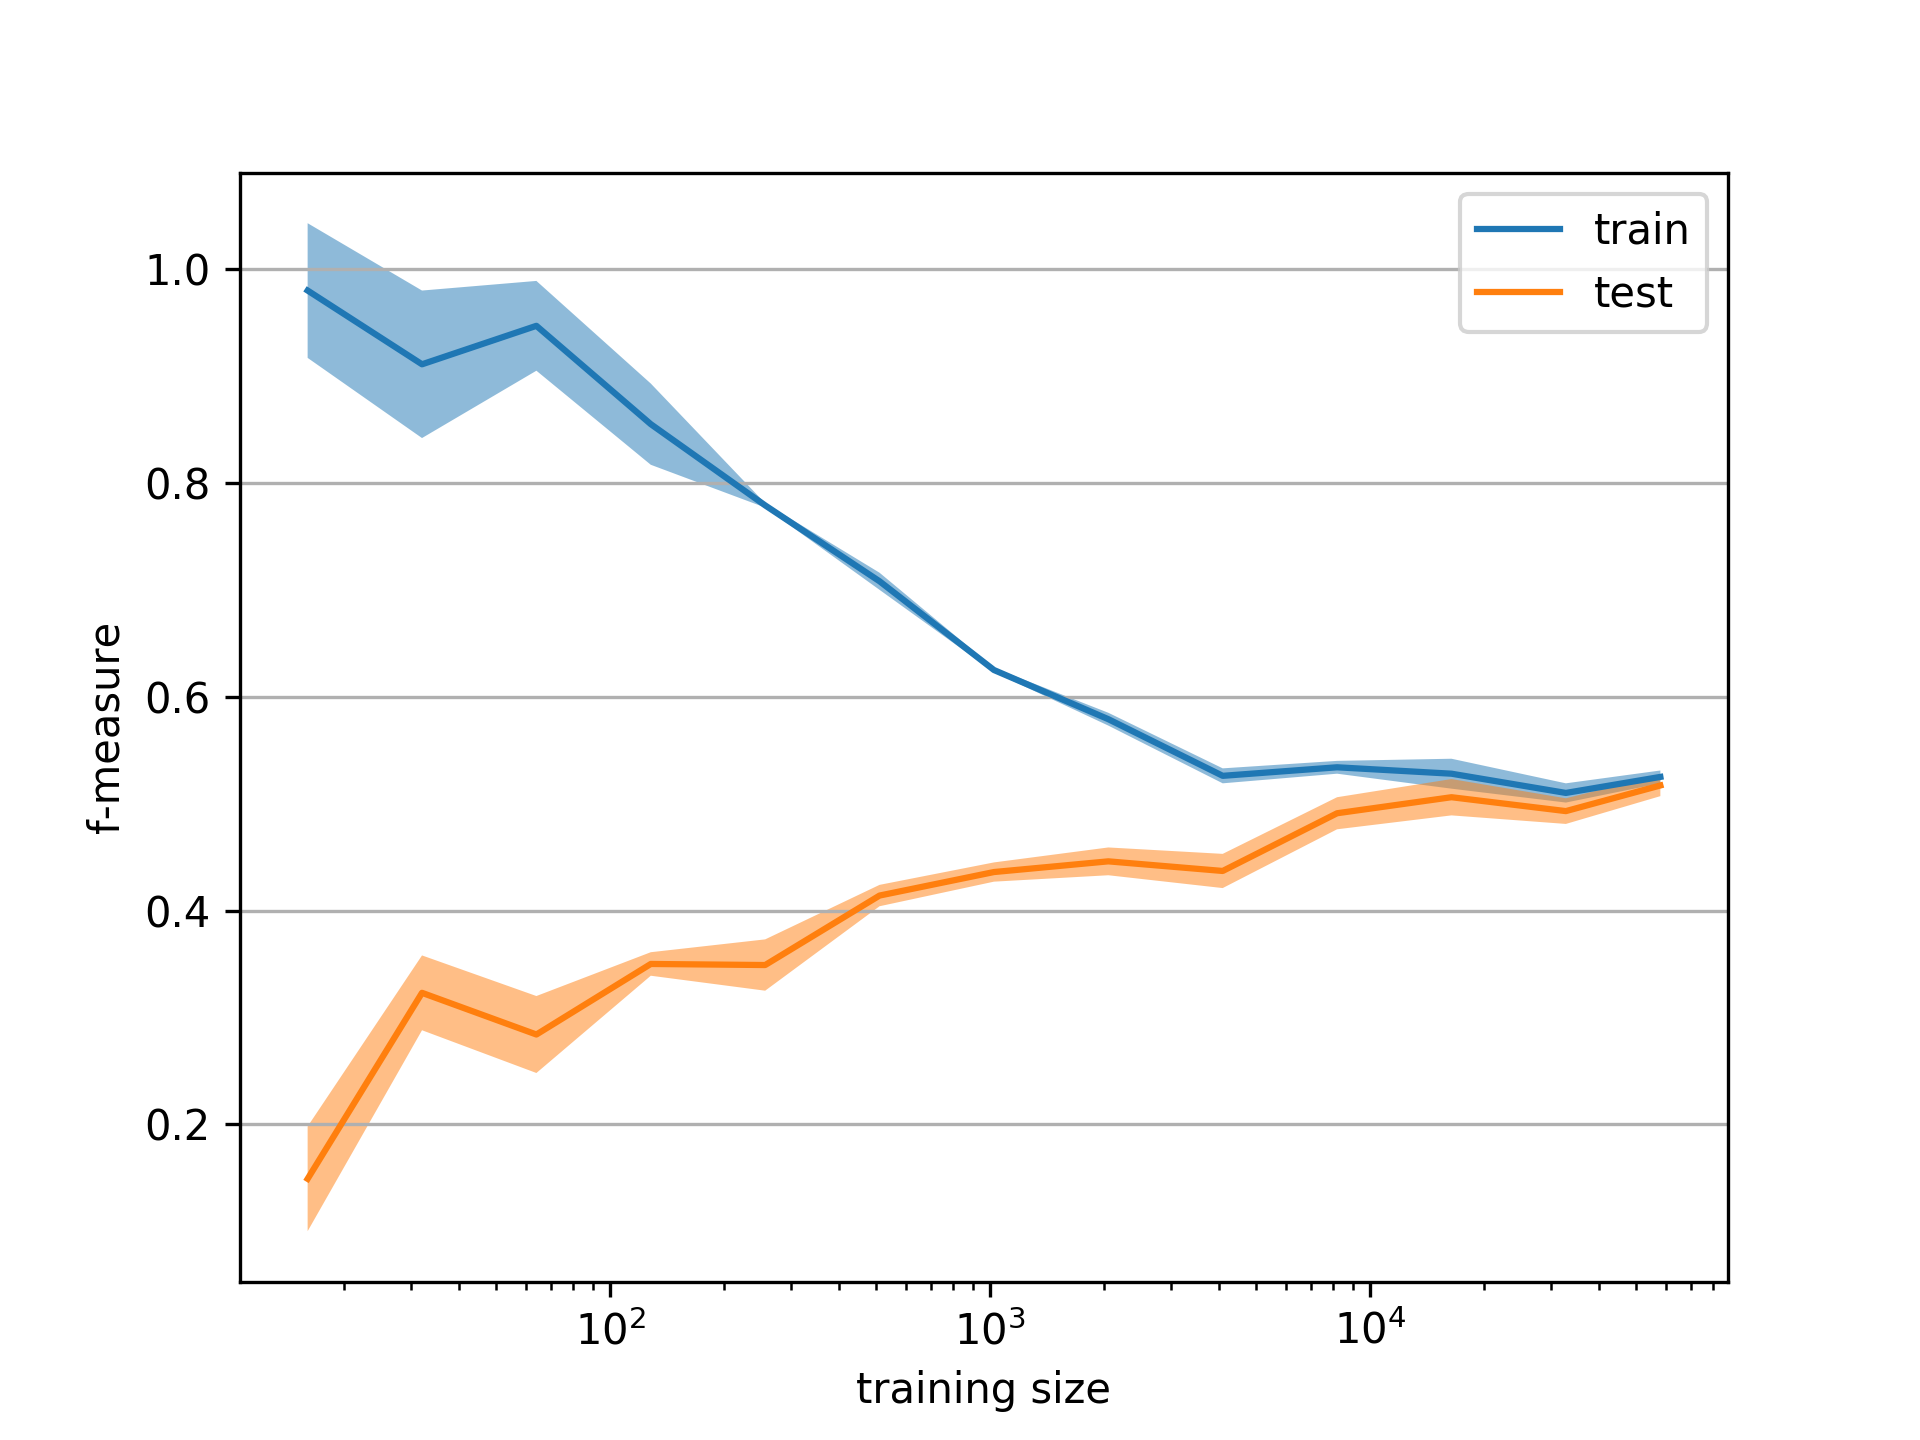
\includegraphics[width=130mm]{figures/lc3_fm.png}
\caption{Learning curves with standard deviation for decision tree --- f-measure}\label{fig:l_curves3_f_measure}
The x axis is log scaled.
\end{figure}
